\section{Training}
\label{s:appendix-b}


\begin{figure}[!htb]
    \centering
    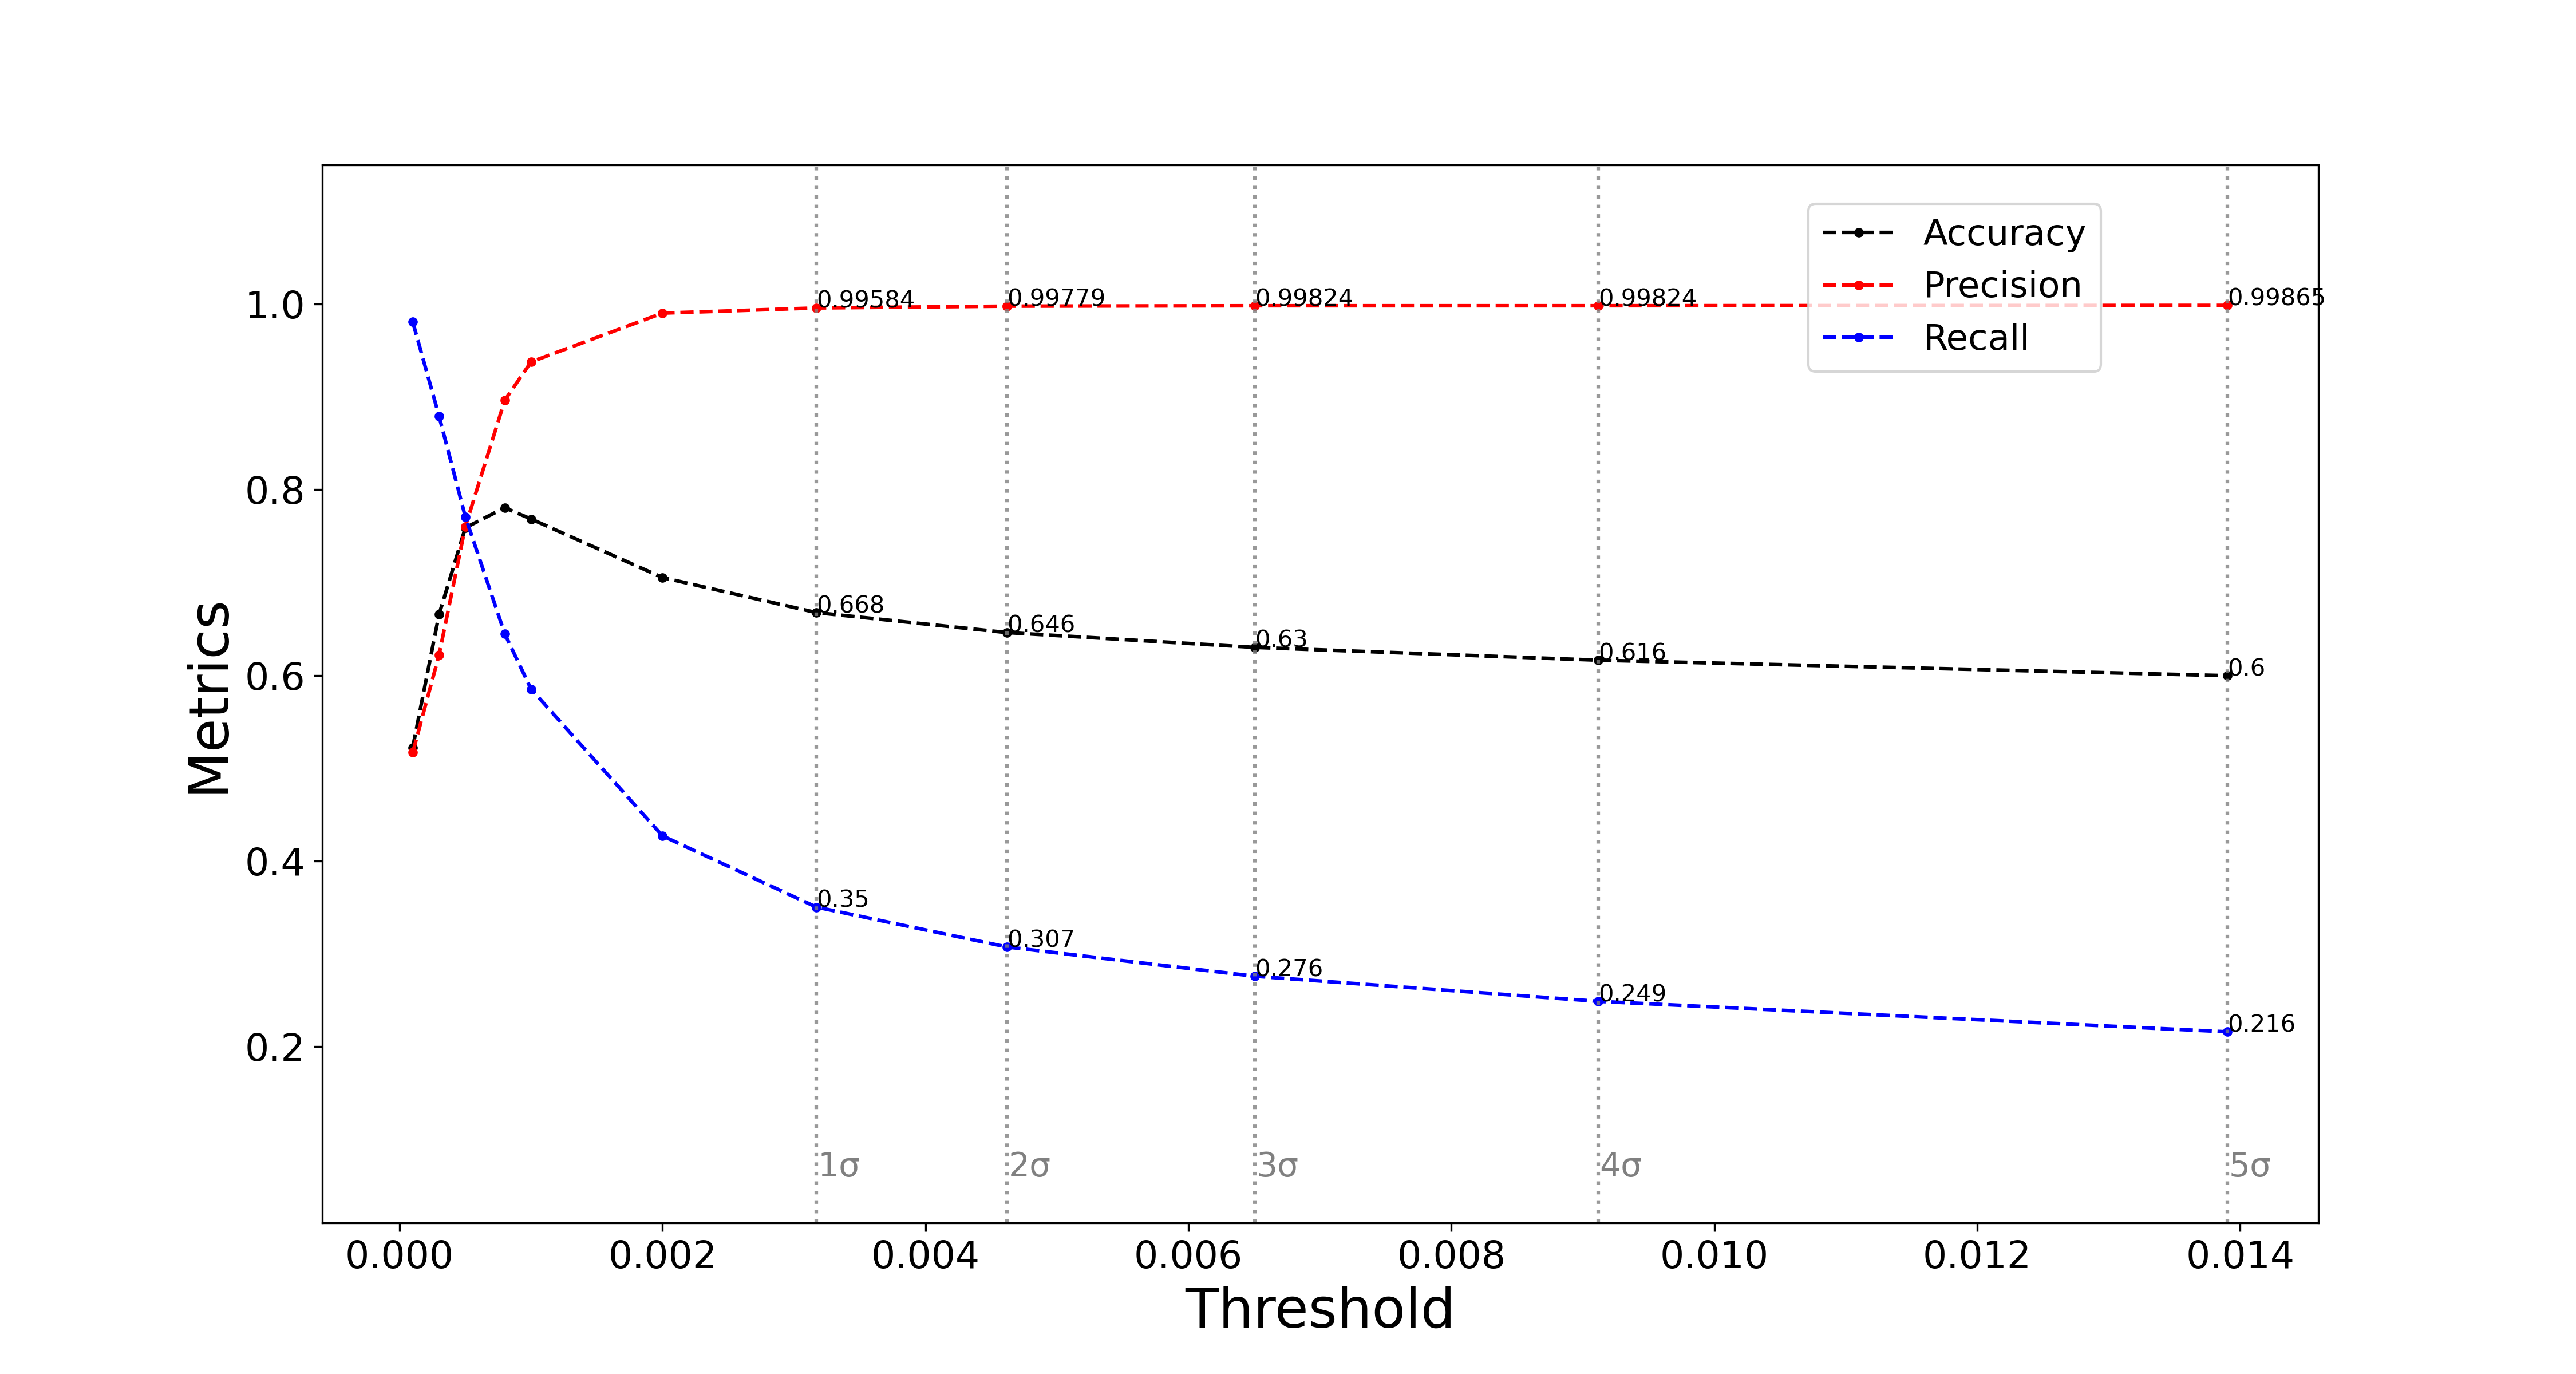
\includegraphics[width=\linewidth]{figures/experiments/metrics/cnn_metrics_test_set_all_itime_5.png}
    \caption{Accuracy, precision and recall curves for the Anomaly Detector with CNN layers in the short term settings (integration time = 5).}
    \label{fig:cnn-metrics-itime-5-appendix}
\end{figure}

\begin{figure}[!htb]
    \centering
    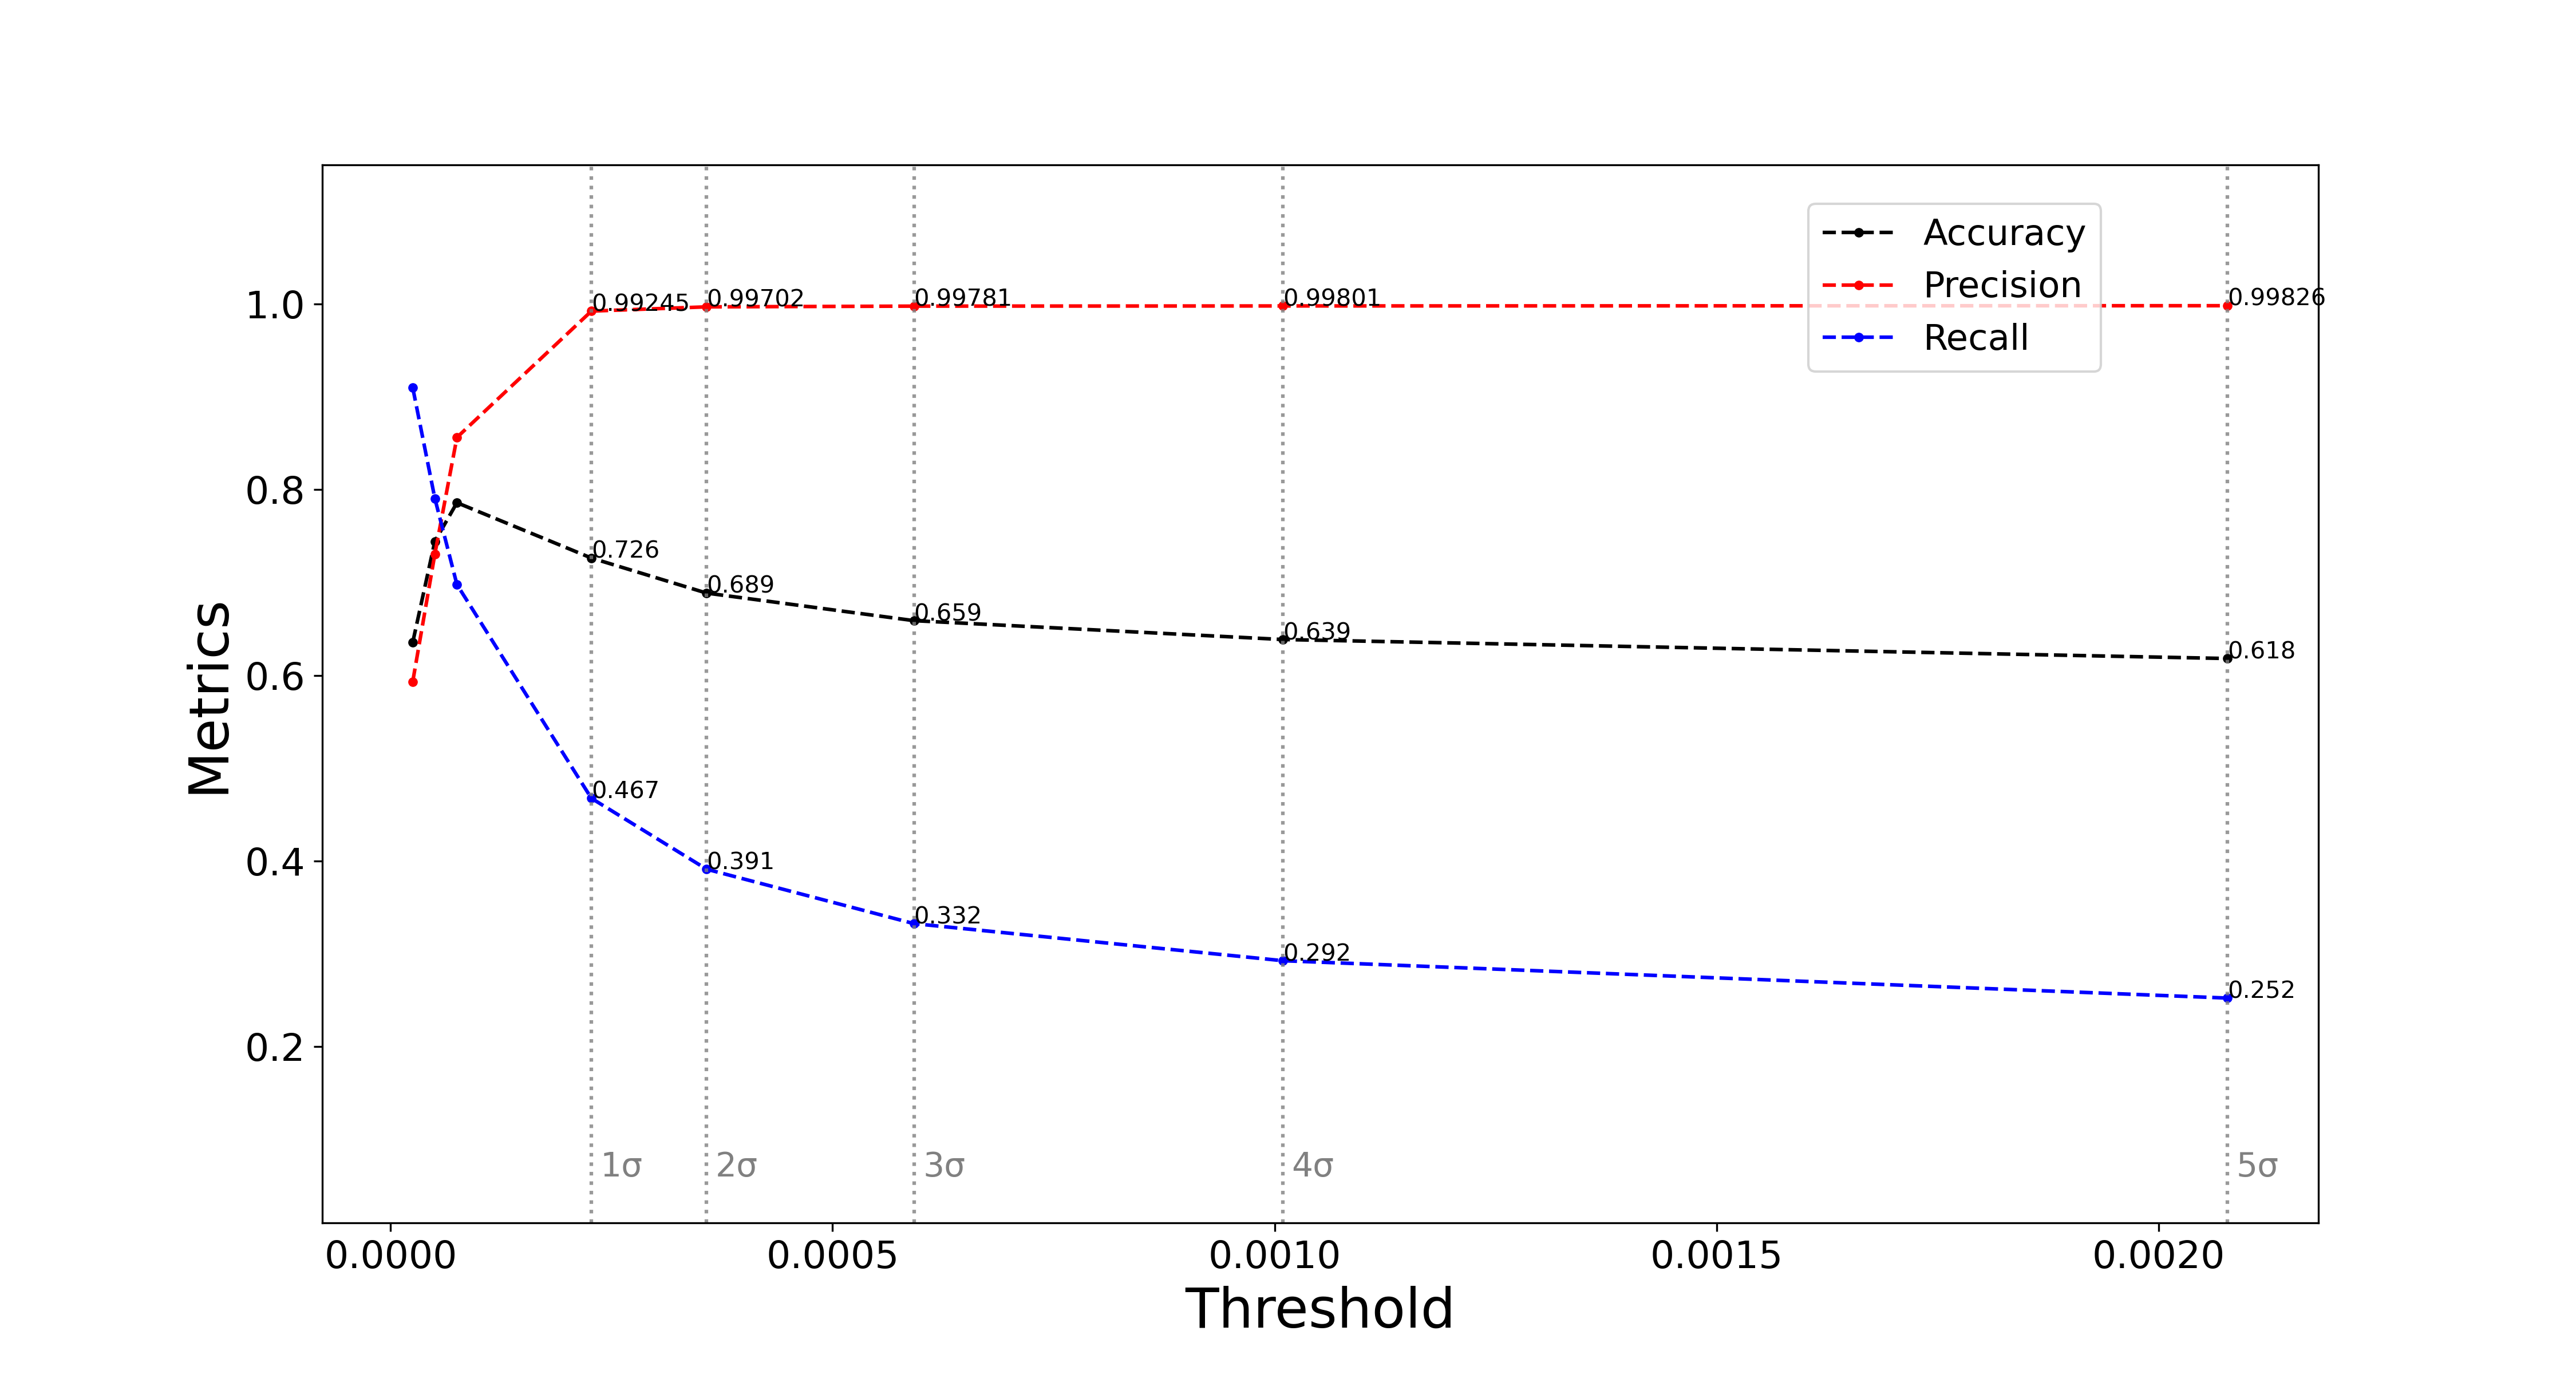
\includegraphics[width=\linewidth]{figures/experiments/metrics/rnn_metrics_test_set_all_itime_5.png}
    \caption{Accuracy, precision and recall curves for the Anomaly Detector with RNN layers in the short term settings (integration time = 5).}
    \label{fig:rnn-metrics-itime-5-appendix}
\end{figure}

\begin{figure}[!htb]
    \centering
    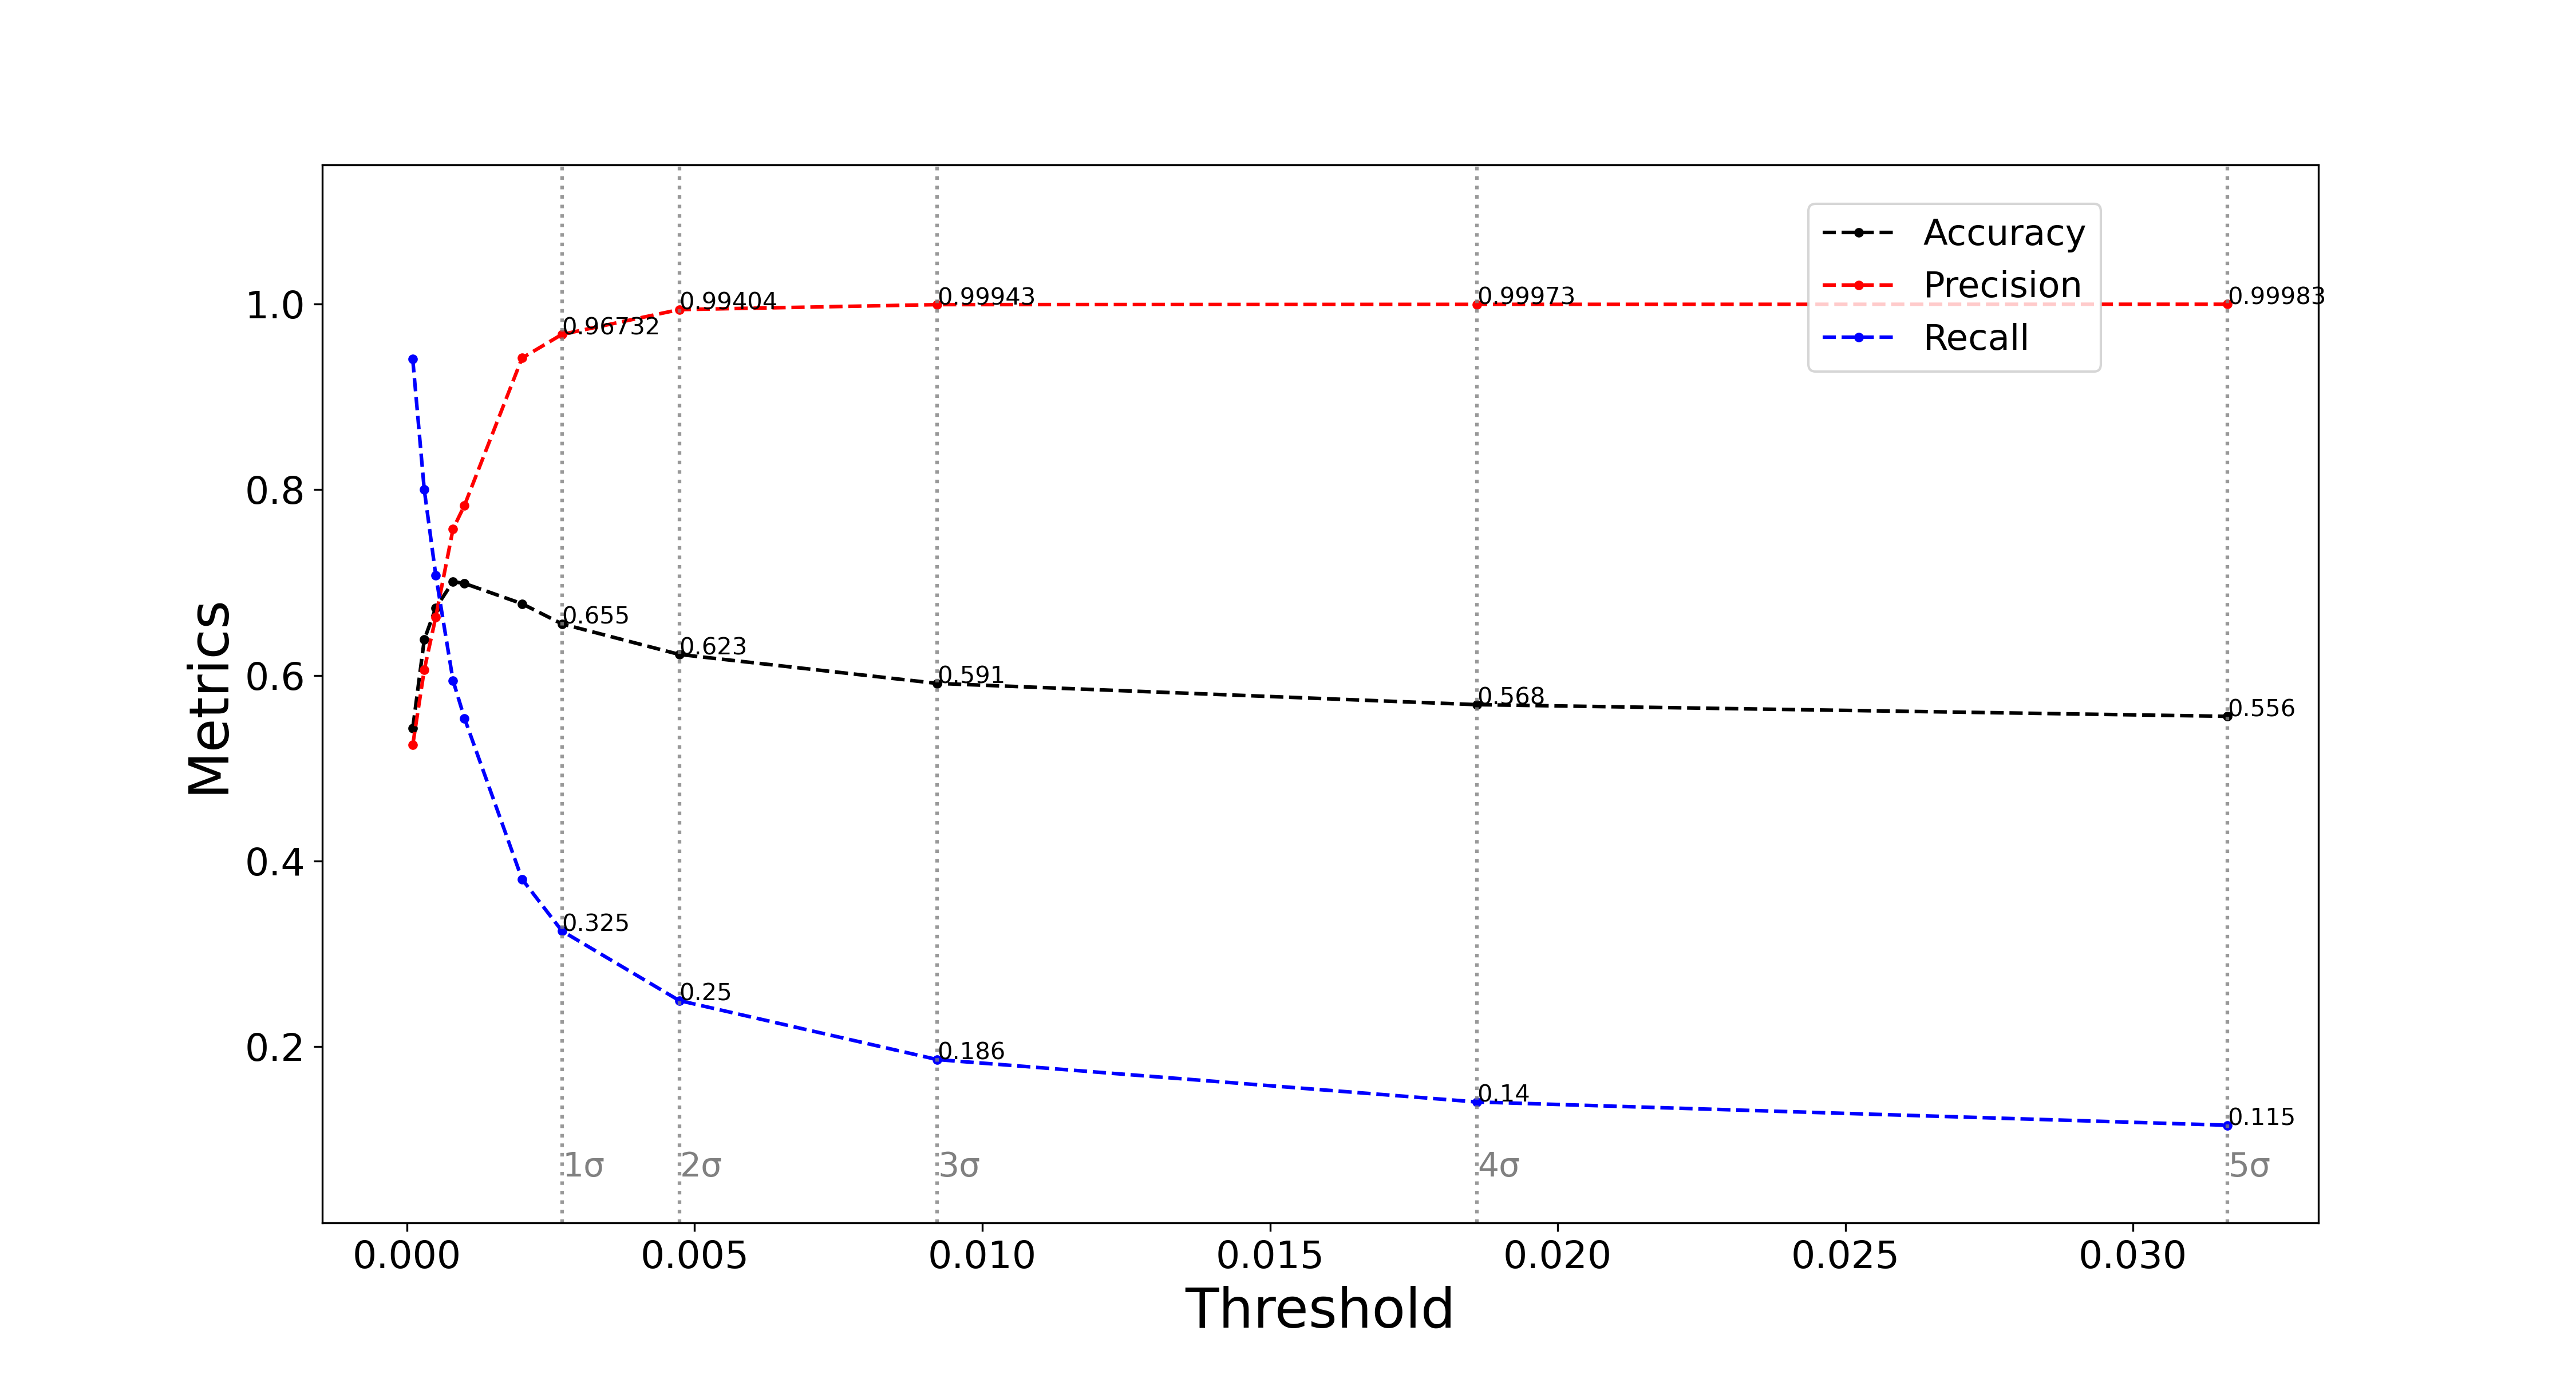
\includegraphics[width=\linewidth]{figures/experiments/metrics/cnn_metrics_test_set_all_itime_1.png}
    \caption{Accuracy, precision and recall curves for the Anomaly Detector with CNN layers in the very short term settings (integration time = 1).}
    \label{fig:cnn-metrics-itime-1-appendix}
\end{figure}

\begin{figure}[!htb]
    \centering
    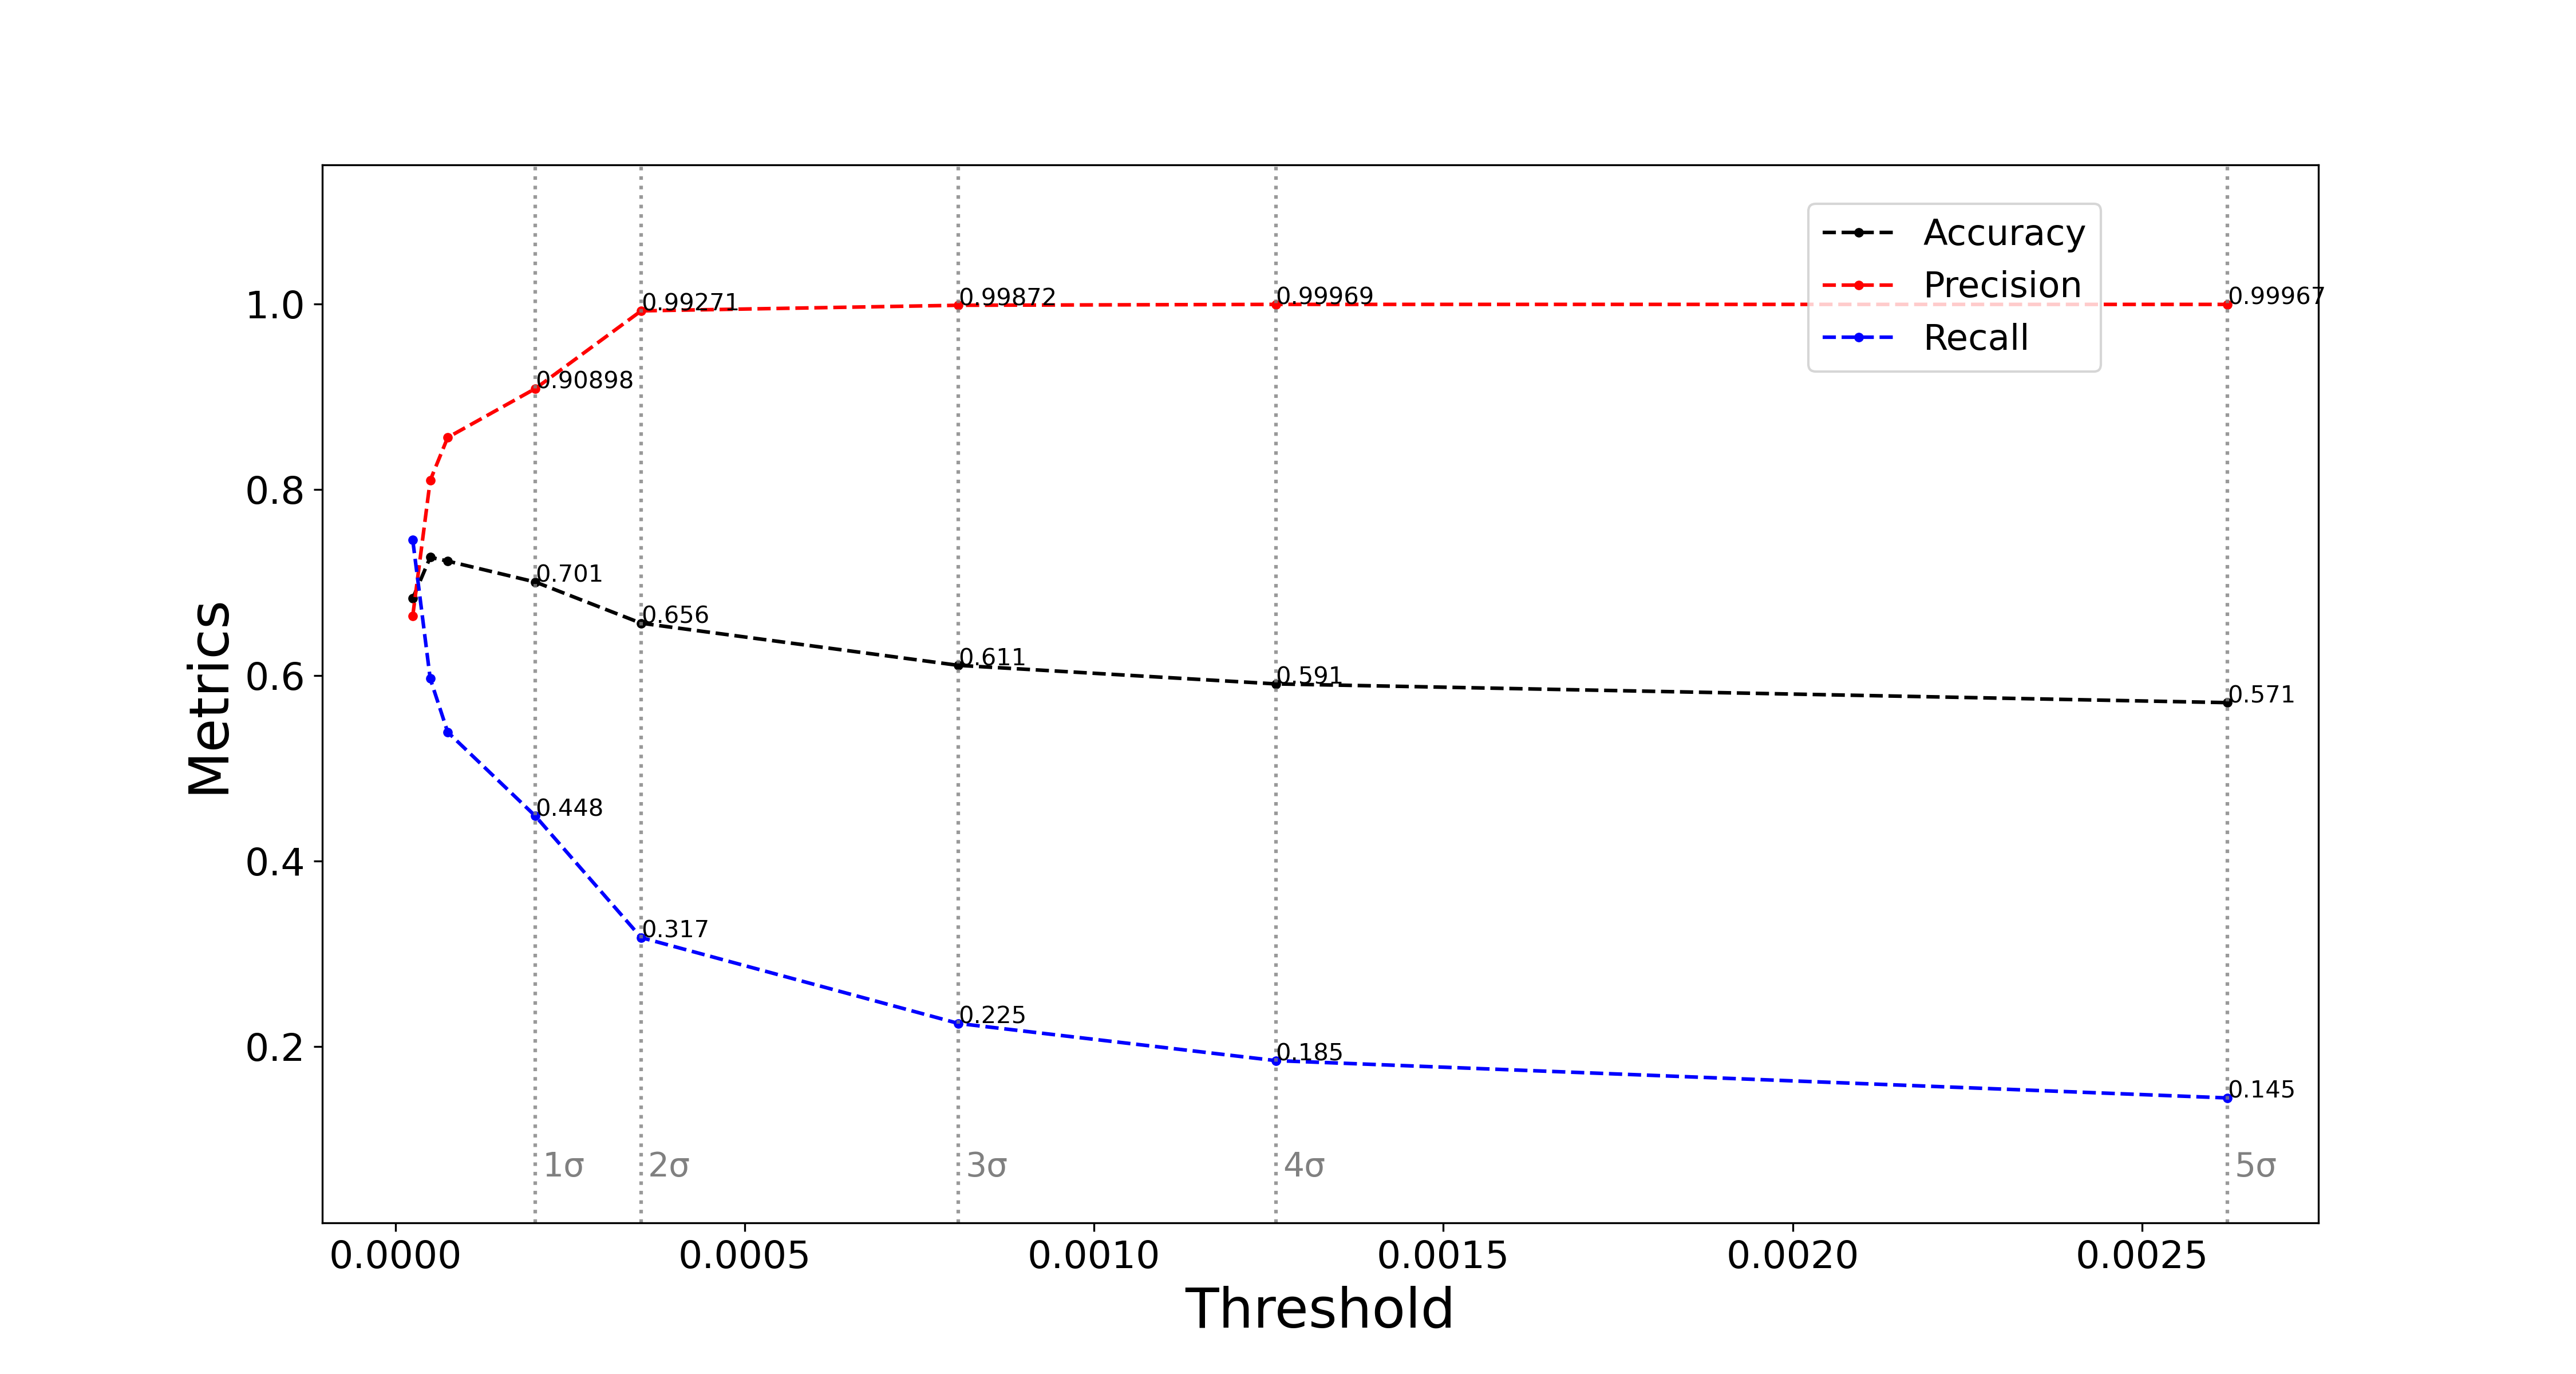
\includegraphics[width=\linewidth]{figures/experiments/metrics/rnn_metrics_test_set_all_itime_1.png}
    \caption{Accuracy, precision and recall curves for the Anomaly Detector with RNN layers in the short term settings (integration time = 1).}
    \label{fig:rnn-metrics-itime-1-appendix}
\end{figure}




\FloatBarrier
\section{}